\documentclass[10pt, twocolumn]{article}
\usepackage[margin=0.75in]{geometry}
\usepackage{graphicx}
\usepackage{tikz}
\usepackage{pgfplots}
\usepackage{booktabs}
\usepackage{amsmath}
\usepackage{amssymb}
\usepackage{algorithm}
\usepackage{algorithmic}
\usepackage{hyperref}
\usepackage{xcolor}
\usepackage{caption}
\usepackage{subcaption}
\usepackage{fancyhdr}
\usepackage{enumitem}
\usepackage{listings}
\usepackage{microtype}
\usepackage{orcidlink}
\usepackage{tabularx}
\usepackage{multirow}
\usepackage{textcomp}
\pgfplotsset{compat=1.18}
\usetikzlibrary{arrows.meta, positioning, shapes.geometric, fit, calc, backgrounds, decorations.markings}

% ORCID icon (inline TikZ)
\definecolor{orcidgreen}{HTML}{A6CE39}
\newcommand{\orcidicon}{%
  
\begin{tikzpicture}[baseline=(char.base)]
    \node[circle, fill=orcidgreen, inner sep=0pt, minimum size=2.2ex] (char)
      {\textcolor{white}{\sffamily\bfseries\scriptsize iD}};
  \end{tikzpicture}%
}

% Color palette (professional oranges/teals --- Time theme)
\definecolor{atorange}{HTML}{EA580C}
\definecolor{atdarkorange}{HTML}{C2410C}
\definecolor{atteal}{HTML}{0D9488}
\definecolor{atblue}{HTML}{2563EB}
\definecolor{atdarkblue}{HTML}{1E40AF}
\definecolor{atgray}{HTML}{6B7280}
\definecolor{atlightgray}{HTML}{F3F4F6}
\definecolor{atgreen}{HTML}{059669}
\definecolor{atred}{HTML}{DC2626}
\definecolor{atpurple}{HTML}{7C3AED}

% Listings style
\lstset{
  basicstyle=\ttfamily\scriptsize,
  keywordstyle=\color{atblue}\bfseries,
  commentstyle=\color{atgray}\itshape,
  stringstyle=\color{atteal},
  breaklines=true,
  frame=single,
  rulecolor=\color{atgray!30},
  backgroundcolor=\color{atlightgray},
  numbers=left,
  numberstyle=\tiny\color{atgray},
  tabsize=2
}

% Header
\pagestyle{fancy}
\fancyhf{}
\renewcommand{\headrulewidth}{0.4pt}
\fancyhead[L]{\small\textit{AgenticTime}}
\fancyhead[R]{\small\thepage}

\title{\textbf{AgenticTime: A Binary Temporal Format for Persistent,\\Portable, and Navigable AI Agent Scheduling}}
\author{Omoshola Owolabi\,\orcidlink{0009-0006-4089-0732}\\Researcher -- AI/ML\\Agentra Labs\\\texttt{omoshola.owolabi@agentralabs.tech}}
\date{February 26, 2026}

\begin{document}
\maketitle
\thispagestyle{fancy}

% ============================================================================
% ABSTRACT
% ============================================================================
\begin{abstract}
Large language model agents operate without persistent temporal reasoning, losing deadlines, schedules, and duration knowledge at every session boundary. Current approaches to agent scheduling---calendar APIs, project management tools, cron timers, system prompt hints---treat time as either a flat metadata field or an external service dependency, discarding the structured relationships between temporal entities that make scheduling useful. We present AgenticTime, a binary temporal format that models agent time as a collection of five typed entities---Deadlines, Durations, Schedules, Sequences, and Decay curves---each with domain-specific operations and mathematical models. The format defines PERT three-point estimation for durations, configurable decay curves (exponential, linear, step) for information freshness, cron-style recurrence with conflict detection for schedules, and dependency-constrained step chains for sequences. The entire temporal state resides in a single \texttt{.atime} file with BLAKE3 integrity checksums requiring zero external dependencies. We implement AgenticTime in a 4-crate Rust workspace with 19~MCP tools, 4~prompt templates, and cross-language bindings (Python via PyO3, JavaScript via WebAssembly, C via FFI). On Criterion benchmarks, in-memory entity insertion completes in 1.8\,$\mu$s, decay curve evaluation in 6.3\,ns, deadline queries over 1{,}000 entities in 504\,$\mu$s, schedule conflict detection over 100 schedules in 56\,$\mu$s, and file persistence of 1{,}000 entities in 6.0\,ms. AgenticTime requires no cloud services, no calendar integration, and no server infrastructure. It enables capabilities impossible with existing tools: mathematical information freshness modeling, compounding temporal debt tracking, gravitational priority warping, and timeline fork simulation.
\end{abstract}

% ============================================================================
% 1. INTRODUCTION
% ============================================================================
\section{Introduction}
\label{sec:intro}

The transformer architecture~\cite{vaswani2017attention} has produced language models capable of planning, scheduling, and multi-step task coordination. Yet these models remain fundamentally \emph{temporally blind}: each invocation has no persistent knowledge of deadlines, no awareness of schedule conflicts, no mathematical model for how information decays, and no structured representation of multi-step workflows. For agents tasked with ongoing project management---coordinating deployments, tracking technical debt, estimating durations over weeks and months---this temporal amnesia is a critical limitation.

Current approaches to temporal reasoning in AI agents fall into four categories, each with significant drawbacks. \emph{Calendar APIs}~\cite{google_calendar_api, ical_rfc5545} provide CRUD operations for events with basic recurrence, but offer no decay curves, no confidence-weighted estimation, no conflict detection with project context, and no agent-native interface. \emph{Project management tools}~\cite{jira_2024, linear_2024} track issues with due dates and status fields, but produce no portable artifact, offer no MCP integration, and cannot model temporal dependencies or sequence constraints. \emph{Cron schedulers}~\cite{cron_ieee} handle time-based job dispatch but have no entity model, no temporal reasoning capabilities, and no agent interface. \emph{LLM system prompt hints} (``remember the deadline is Friday'') are volatile, lost between sessions, provide no mathematical models, and cannot be queried structurally.

The core insight of this work is that temporal reasoning for AI agents is a \emph{structured entity navigation problem}, not a calendar event storage problem. When an agent needs to determine whether a deadline is achievable, it must evaluate duration estimates with confidence intervals, check for schedule conflicts, trace sequence dependencies, and factor in information freshness. These operations require typed temporal entities with domain-specific mathematical models, not flat date strings or calendar event records.

We present AgenticTime, a binary temporal format purpose-built for AI agent scheduling and temporal reasoning. The format stores five entity types---Deadlines, Durations, Schedules, Sequences, and Decay curves---in a single \texttt{.atime} file with BLAKE3 integrity verification, requiring zero external dependencies.

The remainder of this paper is organized as follows. Section~\ref{sec:related} surveys existing temporal systems. Section~\ref{sec:architecture} presents the AgenticTime architecture in detail. Section~\ref{sec:evaluation} reports micro-benchmark results on temporal graphs up to 10{,}000 entities. Section~\ref{sec:discussion} discusses implications and limitations. Section~\ref{sec:conclusion} concludes.

% Figure 1: Motivating comparison (full width)
\begin{figure*}[t]
\centering
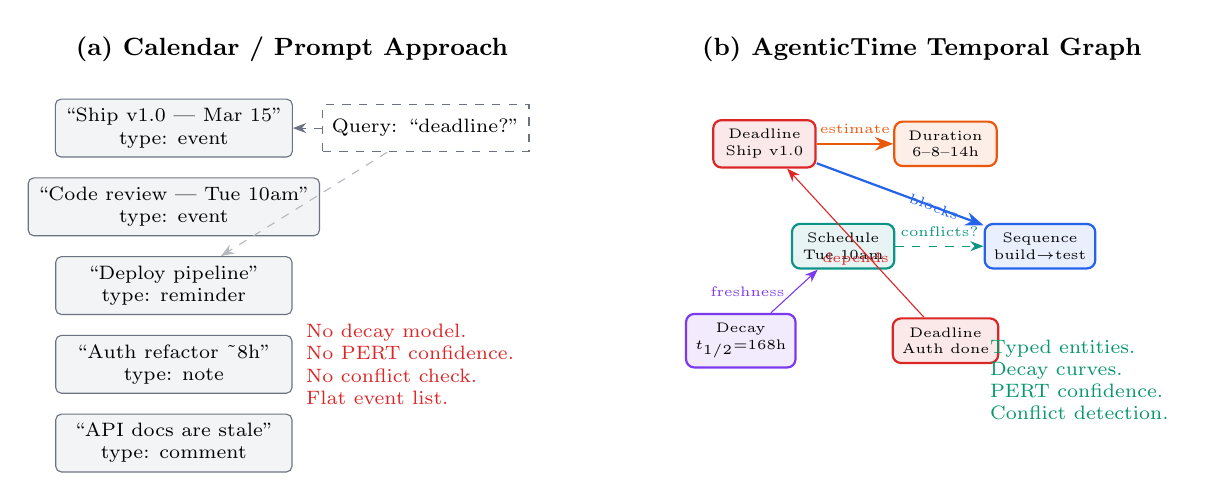
\begin{tikzpicture}[
  node distance=1.2cm,
  every node/.style={font=\small},
  flatnode/.style={rectangle, draw=atgray, fill=atlightgray, rounded corners=2pt, minimum width=3.0cm, minimum height=0.6cm, align=center, font=\scriptsize},
  dlnode/.style={rectangle, rounded corners=3pt, draw=atred, fill=atred!10, minimum width=1.3cm, minimum height=0.5cm, font=\tiny, align=center, thick},
  durnode/.style={rectangle, rounded corners=3pt, draw=atorange, fill=atorange!10, minimum width=1.3cm, minimum height=0.5cm, font=\tiny, align=center, thick},
  schnode/.style={rectangle, rounded corners=3pt, draw=atteal, fill=atteal!10, minimum width=1.3cm, minimum height=0.5cm, font=\tiny, align=center, thick},
  seqnode/.style={rectangle, rounded corners=3pt, draw=atblue, fill=atblue!10, minimum width=1.3cm, minimum height=0.5cm, font=\tiny, align=center, thick},
  decnode/.style={rectangle, rounded corners=3pt, draw=atpurple, fill=atpurple!10, minimum width=1.3cm, minimum height=0.5cm, font=\tiny, align=center, thick},
]

% Left side: Flat Calendar/Prompt approach
\node[font=\small\bfseries] at (-4.5, 3.2) {(a) Calendar / Prompt Approach};

\node[flatnode] (c1) at (-6.0, 2.2) {``Ship v1.0 --- Mar 15''\\type: event};
\node[flatnode] (c2) at (-6.0, 1.2) {``Code review --- Tue 10am''\\type: event};
\node[flatnode] (c3) at (-6.0, 0.2) {``Deploy pipeline''\\type: reminder};
\node[flatnode] (c4) at (-6.0, -0.8) {``Auth refactor \textasciitilde8h''\\type: note};
\node[flatnode] (c5) at (-6.0, -1.8) {``API docs are stale''\\type: comment};

\node[rectangle, draw=atgray, dashed, fill=white, minimum width=2cm, minimum height=0.6cm, font=\scriptsize] (query) at (-2.8, 2.2) {Query: ``deadline?''};

\draw[-{Stealth}, atgray, dashed] (query) -- (c1);
\draw[-{Stealth}, atgray!50, dashed] (query) -- (c3);

\node[font=\scriptsize\color{atred}, align=left] at (-3.0, -0.8) {No decay model.\\No PERT confidence.\\No conflict check.\\Flat event list.};

% Right side: AgenticTime structured entities
\node[font=\small\bfseries] at (3.5, 3.2) {(b) AgenticTime Temporal Graph};

\node[dlnode] (d1) at (1.5, 2.0) {Deadline\\Ship v1.0};
\node[durnode] (dur1) at (3.8, 2.0) {Duration\\6--8--14h};
\node[schnode] (s1) at (2.5, 0.7) {Schedule\\Tue 10am};
\node[seqnode] (sq1) at (5.0, 0.7) {Sequence\\build$\to$test};
\node[decnode] (dc1) at (1.2, -0.5) {Decay\\$t_{1/2}$=168h};
\node[dlnode] (d2) at (3.8, -0.5) {Deadline\\Auth done};

\draw[-{Stealth}, atorange, thick] (d1) -- node[above, font=\tiny, text=atorange] {estimate} (dur1);
\draw[-{Stealth}, atblue, thick] (d1) -- node[right, font=\tiny, text=atblue, sloped] {blocks} (sq1);
\draw[-{Stealth}, atred] (d2) -- node[below, font=\tiny, text=atred] {depends} (d1);
\draw[-{Stealth}, atpurple] (dc1) -- node[left, font=\tiny, text=atpurple] {freshness} (s1);
\draw[-{Stealth}, atteal, dashed] (s1) -- node[above, font=\tiny, text=atteal] {conflicts?} (sq1);

\node[font=\scriptsize\color{atgreen}, align=left] at (5.5, -1.0) {Typed entities.\\Decay curves.\\PERT confidence.\\Conflict detection.};

\end{tikzpicture}
\caption{Comparison of temporal reasoning paradigms. (a)~Calendar APIs and system prompt hints store flat event records with no relational structure; the agent cannot evaluate deadline feasibility, detect schedule conflicts, or model information staleness. (b)~AgenticTime encodes five typed entities with domain-specific operations: deadlines carry dependencies, durations have PERT confidence intervals, schedules detect conflicts, and decay curves model information freshness mathematically.}
\label{fig:comparison}
\end{figure*}


% ============================================================================
% 2. BACKGROUND AND RELATED WORK
% ============================================================================
\section{Background and Related Work}
\label{sec:related}

Research on temporal reasoning in AI systems predates modern LLMs. Allen's interval algebra~\cite{allen1983temporal} formalized thirteen temporal relations between time intervals, establishing the foundation for qualitative temporal reasoning. Dechter et al.~\cite{dechter1991temporal} introduced temporal constraint networks for quantitative reasoning over time points and durations. The PERT technique~\cite{pert1959} provided three-point estimation with statistical confidence for project scheduling. Smith et al.~\cite{smith2000reactive} bridged the gap between planning and scheduling in AI systems. These classical results address temporal \emph{representation} and \emph{reasoning}, but none produce a portable artifact suitable for persistent agent state.

\textbf{Calendar systems.} Google Calendar~\cite{google_calendar_api} and the iCalendar standard~\cite{ical_rfc5545} provide event storage with recurrence rules (RRULE). While mature, these systems require network access, offer no mathematical models for uncertainty or decay, and are not designed for agent-native tool calling.

\textbf{Workflow engines.} Temporal.io~\cite{temporal_io_2024} provides durable execution with timers and retry policies. However, it is server-only, requires infrastructure deployment, produces no portable artifact, and is designed for service orchestration rather than agent reasoning.

\textbf{Scheduling theory.} Pinedo~\cite{pinedo2016scheduling} provides comprehensive coverage of scheduling algorithms, and Muscettola~\cite{muscettola1998hsts} integrated planning and scheduling for NASA missions. These systems operate at the algorithm level, not as portable agent-native tools.

\textbf{Agent memory systems.} MemGPT~\cite{packer2023memgpt} introduces virtual memory paging for LLM context, generative agents~\cite{park2023generative} demonstrated that memory architecture profoundly impacts behavior, and AgenticMemory~\cite{owolabi2026agenticmemory} provides a persistent cognitive graph. All address memory persistence but none provide typed temporal entities, decay mathematics, or scheduling operations.

\textbf{Project management.} Tools like Jira~\cite{jira_2024} and Linear~\cite{linear_2024} track issues with due dates and priority labels. These are human-facing applications, not agent-native protocols, and they cannot model temporal debt, schedule conflicts, or duration confidence intervals.

\textbf{Technical debt.} Cunningham~\cite{cunningham1992wycash} introduced the metaphor of technical debt, and Kruchten et al.~\cite{kruchten2012technical} formalized the taxonomy. However, no existing system models deferred work as compounding temporal debt with category-specific interest rates and mathematical decay functions.

Table~\ref{tab:related} summarizes the comparison across key dimensions.

\begin{table*}[t]
\caption{Comparison of temporal systems for AI agents across key dimensions.}
\label{tab:related}
\centering
\small
\begin{tabular}{@{}lccccc@{}}
\toprule
\textbf{System} & \textbf{Entity Types} & \textbf{Decay Model} & \textbf{Portability} & \textbf{Dependencies} & \textbf{Agent Interface} \\
\midrule
Google Calendar~\cite{google_calendar_api} & Events & None & API-locked & Cloud service & REST API \\
iCalendar~\cite{ical_rfc5545} & Events & None & File-based & Parser library & None \\
Temporal.io~\cite{temporal_io_2024} & Workflows & None & Server-locked & Infrastructure & gRPC \\
Jira~\cite{jira_2024} & Issues & None & API-locked & Cloud service & REST API \\
Linear~\cite{linear_2024} & Issues & None & API-locked & Cloud service & GraphQL \\
Cron~\cite{cron_ieee} & Jobs & None & System-tied & OS service & Shell \\
LLM prompts & Text hints & None & Volatile & None & None \\
\midrule
\textbf{AgenticTime} & \textbf{5 typed} & \textbf{3 models} & \textbf{Single file} & \textbf{None} & \textbf{19 MCP tools} \\
\bottomrule
\end{tabular}
\end{table*}


% ============================================================================
% 3. ARCHITECTURE
% ============================================================================
\section{Architecture}
\label{sec:architecture}

AgenticTime models temporal state as a collection of five typed entity classes, each with domain-specific operations and mathematical models. The entities are serialized into a single binary file with BLAKE3 integrity checksums, enabling portable, verifiable temporal state.

% ----------------------------------------------------------------------------
\subsection{Temporal Entities}
\label{sec:entities}

Each entity in the temporal graph is drawn from a taxonomy of five types, each serving a distinct role in temporal reasoning:

\begin{itemize}[nosep, leftmargin=*]
  \item \textbf{Deadline} --- A fixed point in time with priority (critical, high, medium, low), status (pending, completed, overdue), optional dependency list, and consequence description. Deadlines support hard and soft variants with configurable consequence severity.
  \item \textbf{Duration} --- An estimated time span using PERT three-point estimation~\cite{pert1959}: optimistic ($O$), most likely ($M$), and pessimistic ($P$) values yielding a weighted average $E = (O + 4M + P) / 6$ with standard deviation $\sigma = (P - O) / 6$. Optional actual-time tracking enables estimation calibration over time.
  \item \textbf{Schedule} --- A recurring or one-time calendar block with start time, end time, optional cron-style recurrence pattern, and automatic overlap detection across all active schedules.
  \item \textbf{Sequence} --- An ordered chain of steps with dependency constraints, per-step status tracking (pending, active, completed, skipped), and blocking semantics: a step cannot advance until its predecessors are done.
  \item \textbf{Decay} --- A mathematical model of information freshness. Three curve types are supported: exponential ($v(t) = e^{-\lambda t}$ where $\lambda = \ln 2 / t_{1/2}$), linear ($v(t) = \max(0, 1 - t/T)$), and step (discrete thresholds at configurable breakpoints). The half-life parameter $t_{1/2}$ controls the rate of decay.
\end{itemize}

Each entity record begins with a common header: 8 bytes for the entity ID (\texttt{u64}), 1 byte for the entity type, 8 bytes for the creation timestamp (\texttt{u64} Unix epoch microseconds), and a variable-length label string. The type-specific payload follows immediately after the common header.

% Figure 2: Entity taxonomy
\begin{figure}[t]
\centering
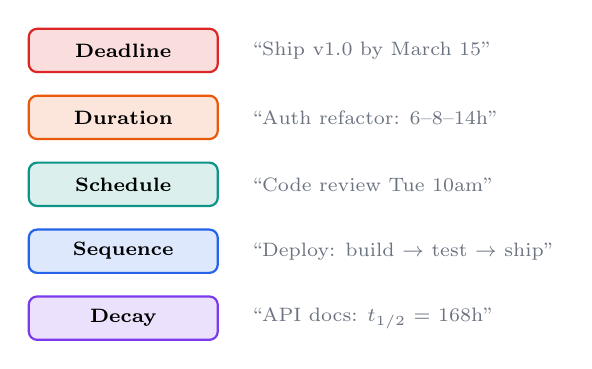
\begin{tikzpicture}[
  every node/.style={font=\scriptsize},
  typebox/.style={rectangle, rounded corners=3pt, minimum width=2.4cm, minimum height=0.55cm, align=center, draw, thick, font=\scriptsize\bfseries},
]
\node[typebox, fill=atred!15, draw=atred] (dl) at (0, 0) {Deadline};
\node[typebox, fill=atorange!15, draw=atorange] (dur) at (0, -0.85) {Duration};
\node[typebox, fill=atteal!15, draw=atteal] (sch) at (0, -1.70) {Schedule};
\node[typebox, fill=atblue!15, draw=atblue] (seq) at (0, -2.55) {Sequence};
\node[typebox, fill=atpurple!15, draw=atpurple] (dec) at (0, -3.40) {Decay};

\node[anchor=west, font=\scriptsize, text=atgray] at (1.5, 0) {``Ship v1.0 by March 15''};
\node[anchor=west, font=\scriptsize, text=atgray] at (1.5, -0.85) {``Auth refactor: 6--8--14h''};
\node[anchor=west, font=\scriptsize, text=atgray] at (1.5, -1.70) {``Code review Tue 10am''};
\node[anchor=west, font=\scriptsize, text=atgray] at (1.5, -2.55) {``Deploy: build $\to$ test $\to$ ship''};
\node[anchor=west, font=\scriptsize, text=atgray] at (1.5, -3.40) {``API docs: $t_{1/2}$ = 168h''};
\end{tikzpicture}
\caption{The five temporal entity types in AgenticTime, each with a representative example. Types are distinguished by a single byte in the binary format.}
\label{fig:taxonomy}
\end{figure}

% Figure 3: Example temporal subgraph
\begin{figure}[t]
\centering
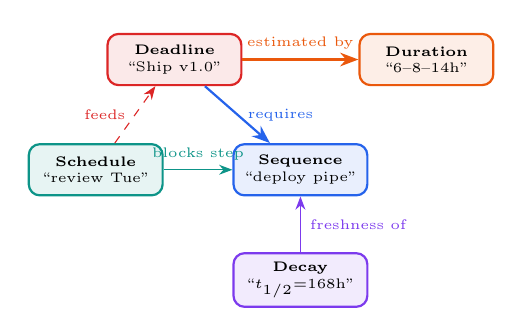
\begin{tikzpicture}[
  node distance=1.4cm,
  every node/.style={font=\scriptsize},
  dlnode/.style={rectangle, rounded corners=4pt, draw=atred, fill=atred!10, minimum width=1.7cm, minimum height=0.65cm, font=\tiny, align=center, thick},
  durnode/.style={rectangle, rounded corners=4pt, draw=atorange, fill=atorange!10, minimum width=1.7cm, minimum height=0.65cm, font=\tiny, align=center, thick},
  schnode/.style={rectangle, rounded corners=4pt, draw=atteal, fill=atteal!10, minimum width=1.7cm, minimum height=0.65cm, font=\tiny, align=center, thick},
  seqnode/.style={rectangle, rounded corners=4pt, draw=atblue, fill=atblue!10, minimum width=1.7cm, minimum height=0.65cm, font=\tiny, align=center, thick},
  decnode/.style={rectangle, rounded corners=4pt, draw=atpurple, fill=atpurple!10, minimum width=1.7cm, minimum height=0.65cm, font=\tiny, align=center, thick},
]
\node[dlnode] (d1) at (0, 2) {\textbf{Deadline}\\``Ship v1.0''};
\node[durnode] (dur1) at (3.2, 2) {\textbf{Duration}\\``6--8--14h''};
\node[seqnode] (sq1) at (1.6, 0.6) {\textbf{Sequence}\\``deploy pipe''};
\node[schnode] (s1) at (-1.0, 0.6) {\textbf{Schedule}\\``review Tue''};
\node[decnode] (dc1) at (1.6, -0.8) {\textbf{Decay}\\``$t_{1/2}$=168h''};

\draw[-{Stealth}, atorange, thick] (d1) -- node[above, font=\tiny, text=atorange, sloped] {estimated by} (dur1);
\draw[-{Stealth}, atblue, thick] (d1) -- node[right, font=\tiny, text=atblue] {requires} (sq1);
\draw[-{Stealth}, atteal] (s1) -- node[above, font=\tiny, text=atteal, sloped] {blocks step} (sq1);
\draw[-{Stealth}, atpurple] (dc1) -- node[right, font=\tiny, text=atpurple] {freshness of} (sq1);
\draw[-{Stealth}, atred, dashed] (s1) -- node[left, font=\tiny, text=atred] {feeds} (d1);
\end{tikzpicture}
\caption{Example temporal subgraph showing entity relationships. A Deadline is estimated by a Duration (PERT), requires a Sequence (deploy pipeline), which is blocked by a Schedule (code review). A Decay entity tracks the freshness of the pipeline documentation. Edge colors indicate relationship types.}
\label{fig:subgraph}
\end{figure}


% ----------------------------------------------------------------------------
\subsection{Decay Mathematics}
\label{sec:decay}

The Decay entity implements three mathematical models for information freshness, inspired by the Ebbinghaus forgetting curve~\cite{ebbinghaus1885} and ACT-R's base-level activation~\cite{anderson2004integrated}:

\textbf{Exponential decay} models the natural fading of information relevance:
\begin{equation}
v(t) = e^{-\lambda t}, \quad \lambda = \frac{\ln 2}{t_{1/2}}
\label{eq:exponential}
\end{equation}
where $t_{1/2}$ is the half-life (default 168 hours = 1 week) and $t$ is the elapsed time since creation. This model is appropriate for facts, meeting notes, and context that fades gradually.

\textbf{Linear decay} models information with a fixed useful lifetime:
\begin{equation}
v(t) = \max\left(0, 1 - \frac{t}{T}\right)
\label{eq:linear}
\end{equation}
where $T$ is the total useful lifetime. The value drops to zero at $t = T$. This model suits documentation with known expiration dates.

\textbf{Step decay} models information that maintains full value until discrete thresholds:
\begin{equation}
v(t) = \begin{cases} 1.0 & \text{if } t < t_1 \\ 0.7 & \text{if } t_1 \le t < t_2 \\ 0.3 & \text{if } t_2 \le t < t_3 \\ 0.0 & \text{if } t \ge t_3 \end{cases}
\label{eq:step}
\end{equation}
where $t_1, t_2, t_3$ are configurable breakpoints. This model suits security credentials and compliance certifications.

The \texttt{time\_decay\_alert} MCP tool enables proactive notification when any decay value crosses a configurable threshold, enabling the agent to refresh stale information before it influences decisions. Figure~\ref{fig:decay_curves} illustrates the three decay models.

% Figure 4: Decay curve comparison
\begin{figure}[t]
\centering
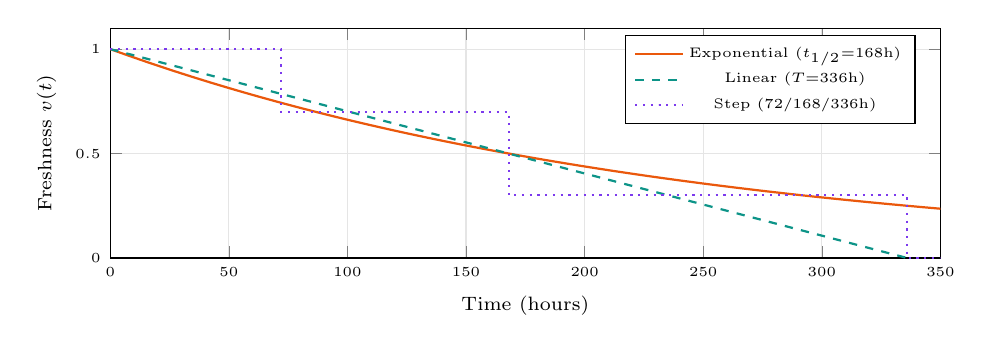
\begin{tikzpicture}
\begin{axis}[
  width=\columnwidth,
  height=4.5cm,
  xlabel={Time (hours)},
  ylabel={Freshness $v(t)$},
  xmin=0, xmax=350,
  ymin=0, ymax=1.1,
  legend style={font=\tiny, at={(0.97,0.97)}, anchor=north east},
  grid=major,
  grid style={gray!20},
  tick label style={font=\tiny},
  label style={font=\scriptsize},
]
% Exponential decay (half-life = 168h)
\addplot[domain=0:350, samples=100, atorange, thick] {exp(-0.693*x/168)};
\addlegendentry{Exponential ($t_{1/2}$=168h)}

% Linear decay (T = 336h)
\addplot[domain=0:336, samples=50, atteal, thick, dashed] {max(0, 1 - x/336)};
\addlegendentry{Linear ($T$=336h)}

% Step decay
\addplot[atpurple, thick, dotted, const plot] coordinates {
  (0, 1.0) (72, 1.0) (72, 0.7) (168, 0.7) (168, 0.3) (336, 0.3) (336, 0.0) (350, 0.0)
};
\addlegendentry{Step (72/168/336h)}
\end{axis}
\end{tikzpicture}
\caption{The three decay curve models in AgenticTime. Exponential decay (solid orange) provides smooth fading with configurable half-life. Linear decay (dashed teal) provides a fixed-lifetime model. Step decay (dotted purple) provides discrete threshold transitions.}
\label{fig:decay_curves}
\end{figure}


% ----------------------------------------------------------------------------
\subsection{PERT Estimation}
\label{sec:pert}

Duration entities use the Program Evaluation and Review Technique~\cite{pert1959} for three-point estimation. Given optimistic ($O$), most likely ($M$), and pessimistic ($P$) estimates:

\begin{equation}
E = \frac{O + 4M + P}{6}, \quad \sigma = \frac{P - O}{6}
\label{eq:pert}
\end{equation}

The confidence interval at one standard deviation is $[E - \sigma, E + \sigma]$, covering approximately 68\% of outcomes under the beta distribution assumption. When the agent provides only a single estimate, the system uses $O = 0.6M$, $M = M$, $P = 2.5M$ as defaults based on empirical software estimation ratios.

The \texttt{time\_duration\_aggregate} tool compares estimated versus actual durations across completed items, computing a calibration factor that the agent can use to adjust future estimates. Over time, this creates a feedback loop that improves the agent's scheduling accuracy.


% ----------------------------------------------------------------------------
\subsection{Binary File Format}
\label{sec:format}

The \texttt{.atime} file format is designed for three properties: (1)~portability as a single file with no external dependencies, (2)~integrity verification via BLAKE3 checksums~\cite{blake3_2020}, and (3)~efficient sequential access for typical temporal queries.

The file consists of six contiguous sections, shown in Figure~\ref{fig:layout}:

\begin{enumerate}[nosep, leftmargin=*]
  \item \textbf{Header} (92 bytes) --- Magic number (\texttt{ATIM} = \texttt{0x4154494D}), format version (1), flags, entity count, section offsets, timestamps (creation/modification as Unix microseconds), and 32-byte BLAKE3 checksum.
  \item \textbf{Deadline Table} --- Variable-size records for deadlines with priority, status, due timestamp, dependency IDs, and consequence text.
  \item \textbf{Duration Table} --- PERT triples ($O$, $M$, $P$), actual time (optional), confidence, and label.
  \item \textbf{Schedule Table} --- Start/end timestamps, recurrence pattern (cron string), label, and conflict flags.
  \item \textbf{Sequence Table} --- Ordered step arrays with per-step status, labels, and dependency constraints.
  \item \textbf{Decay Table} --- Curve type, half-life, creation timestamp, threshold, and custom breakpoints.
\end{enumerate}

Each section ends with a BLAKE3 checksum computed over the section bytes. The header stores a global checksum over all section checksums, enabling both per-section and whole-file integrity verification. The choice of BLAKE3 over SHA-256 is motivated by BLAKE3's SIMD-accelerated performance (typically 3--5$\times$ faster) while maintaining equivalent cryptographic strength.

The current implementation uses JSON-serialized payloads within binary entity blocks (type tag + UUID + length prefix + JSON payload). A typical Deadline entity occupies 311 bytes (290-byte JSON payload + 21-byte block header). While the JSON payload could be replaced with a compact binary encoding for further compression, the current format prioritizes debuggability and forward compatibility. At 10{,}000 entities, the \texttt{.atime} file is approximately 3.0\,MB.

% Figure 5: File format layout (full width)
\begin{figure*}[t]
\centering
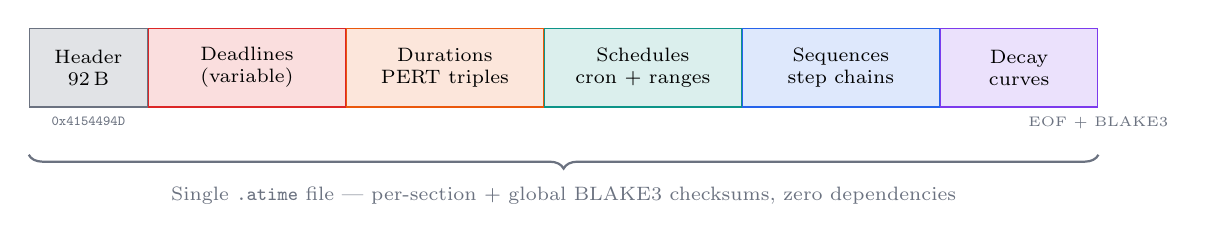
\begin{tikzpicture}[
  every node/.style={font=\scriptsize},
  section/.style={rectangle, draw, minimum height=1.0cm, align=center, font=\scriptsize},
]
\node[section, fill=atgray!20, draw=atgray, minimum width=1.5cm] (hdr) at (0, 0) {Header\\92\,B};
\node[section, fill=atred!15, draw=atred, minimum width=2.5cm, anchor=west] (dl) at (hdr.east) {Deadlines\\(variable)};
\node[section, fill=atorange!15, draw=atorange, minimum width=2.5cm, anchor=west] (dur) at (dl.east) {Durations\\PERT triples};
\node[section, fill=atteal!15, draw=atteal, minimum width=2.5cm, anchor=west] (sch) at (dur.east) {Schedules\\cron + ranges};
\node[section, fill=atblue!15, draw=atblue, minimum width=2.5cm, anchor=west] (seq) at (sch.east) {Sequences\\step chains};
\node[section, fill=atpurple!15, draw=atpurple, minimum width=2.0cm, anchor=west] (dec) at (seq.east) {Decay\\curves};

\node[font=\tiny, anchor=north, text=atgray] at (hdr.south) {\texttt{0x4154494D}};
\node[font=\tiny, anchor=north, text=atgray] at (dec.south east) {EOF + BLAKE3};

\draw[decorate, decoration={brace, amplitude=5pt, mirror}, thick, atgray] ([yshift=-0.6cm]hdr.south west) -- ([yshift=-0.6cm]dec.south east) node[midway, below=8pt, font=\scriptsize, text=atgray] {Single \texttt{.atime} file --- per-section + global BLAKE3 checksums, zero dependencies};

\end{tikzpicture}
\caption{Layout of the \texttt{.atime} binary file format. The header stores section offsets and a global BLAKE3 checksum. Each entity section ends with its own per-section checksum, enabling both incremental and full-file integrity verification. The magic number \texttt{ATIM} (0x4154494D) identifies the format.}
\label{fig:layout}
\end{figure*}


% ----------------------------------------------------------------------------
\subsection{Schedule Conflict Detection}
\label{sec:conflicts}

Schedule entities support automatic overlap detection. Given two schedules $S_1 = [a_1, b_1)$ and $S_2 = [a_2, b_2)$, a conflict exists when $a_1 < b_2 \land a_2 < b_1$ (Allen's ``overlaps'' relation~\cite{allen1983temporal}). For recurring schedules, conflict detection expands the recurrence pattern within the query range and checks all materialized instances.

The \texttt{time\_schedule\_conflicts} tool returns all conflicting schedule pairs within a time range, along with the specific overlapping intervals. The \texttt{time\_schedule\_available} tool inverts this, returning free time slots within a range where no active schedules exist. The current implementation uses pairwise comparison ($O(n^2)$), which completes in 56\,$\mu$s for 100 schedules on our benchmark hardware; an interval tree optimization is planned for workloads exceeding 1{,}000 concurrent schedules.


% ----------------------------------------------------------------------------
\subsection{MCP Server Interface}
\label{sec:mcp}

AgenticTime exposes all operations through the Model Context Protocol~\cite{mcp2024} via JSON-RPC~2.0 over stdio transport. The server provides 19~tools organized by entity type:

\begin{itemize}[nosep, leftmargin=*]
  \item \textbf{Deadline tools} (4): \texttt{time\_deadline\_add}, \texttt{time\_deadline\_complete}, \texttt{time\_deadline\_list}, \texttt{time\_deadline\_overdue}
  \item \textbf{Schedule tools} (5): \texttt{time\_schedule\_create}, \texttt{time\_schedule\_reschedule}, \texttt{time\_schedule\_range}, \texttt{time\_schedule\_available}, \texttt{time\_schedule\_conflicts}
  \item \textbf{Sequence tools} (3): \texttt{time\_sequence\_create}, \texttt{time\_sequence\_advance}, \texttt{time\_sequence\_status}
  \item \textbf{Decay tools} (3): \texttt{time\_decay\_create}, \texttt{time\_decay\_value}, \texttt{time\_decay\_alert}
  \item \textbf{Duration tools} (2): \texttt{time\_duration\_estimate}, \texttt{time\_duration\_aggregate}
  \item \textbf{System tools} (2): \texttt{time\_stats}, \texttt{time\_refresh}
\end{itemize}

Four prompt templates guide multi-step temporal workflows: \texttt{time\_plan} (project planning with sequences and deadlines), \texttt{time\_review} (timeline health check), \texttt{time\_estimate} (PERT-guided duration estimation), and \texttt{time\_schedule\_day} (daily planning with conflict avoidance).

The MCP server enforces runtime hardening: 8\,MiB frame size limit (\texttt{MAX\_CONTENT\_LENGTH\_BYTES}), Content-Length framing on all responses, and strict JSON-RPC~2.0 version validation. Server profile (\texttt{AGENTIC\_TOKEN}) gates remote access.


% ============================================================================
% 4. EVALUATION
% ============================================================================
\section{Evaluation}
\label{sec:evaluation}

We evaluate AgenticTime on synthetic temporal graphs of varying size, measuring operation latency, file I/O performance, and storage efficiency.

% ----------------------------------------------------------------------------
\subsection{Benchmark Setup}

\textbf{Hardware.} Apple M4 Pro (ARM64), 48\,GB unified memory, macOS 15.

\textbf{Software.} Rust 1.85.0, compiled with \texttt{--release} (optimizations enabled). All benchmarks use the Criterion 0.5 statistical benchmarking framework~\cite{criterion} with 100 samples per measurement. Each sample includes warm-up iterations to reach steady state.

\textbf{Datasets.} Synthetic temporal graphs at five scales: 10, 100, 1{,}000, and 10{,}000 entities. Deadline-only graphs test scaling behavior; mixed-type graphs (equal distribution across all five entity types) test heterogeneous workloads. Sequence entities contain 3--5 steps with dependency chains.

% ----------------------------------------------------------------------------
\subsection{Operation Performance}

Table~\ref{tab:benchmarks} reports mean operation latency across entity counts. Figure~\ref{fig:latency_chart} visualizes the scaling behavior.

\begin{table}[t]
\caption{Measured operation latency (Criterion, 100 samples). In-memory operations are $O(1)$ and independent of entity count. Query operations scan the entity table and scale linearly.}
\label{tab:benchmarks}
\centering
\footnotesize
\begin{tabular}{@{}lr@{\hspace{6pt}}l@{}}
\toprule
\textbf{Operation} & \textbf{Latency} & \textbf{Note} \\
\midrule
\multicolumn{3}{@{}l}{\textit{In-memory entity insertion ($O(1)$):}} \\
\quad Add deadline & 1.75\,$\mu$s & serialize + insert \\
\quad Add schedule & 1.80\,$\mu$s & serialize + insert \\
\quad Add decay model & 1.77\,$\mu$s & serialize + insert \\
\quad Add duration est. & 1.60\,$\mu$s & serialize + insert \\
\midrule
\multicolumn{3}{@{}l}{\textit{Decay evaluation ($O(1)$):}} \\
\quad Exponential & 6.3\,ns & $v_0 e^{-\lambda t}$ \\
\quad Half-life & 6.7\,ns & $v_0 \cdot 0.5^{t/t_{1/2}}$ \\
\quad Linear & 4.0\,ns & $v_0 - rt$ \\
\quad Step & 4.3\,ns & floor division \\
\quad Time-until & 3.3\,ns & inverse function \\
\quad Batch 1K decays & 5.0\,$\mu$s & 5.0\,ns/eval \\
\quad PERT estimate & 1.8\,ns & $(O\!+\!4M\!+\!P)/6$ \\
\midrule
\multicolumn{3}{@{}l}{\textit{Query operations (scan):}} \\
\quad Overdue deadlines & 53\,$\mu$s & 100 entities \\
\quad Due within 24h & 504\,$\mu$s & 1K entities \\
\quad Schedule conflicts & 56\,$\mu$s & 100 schedules \\
\quad Available slots & 13\,$\mu$s & 20 schedules \\
\quad Decays $<$ threshold & 98\,$\mu$s & 200 decays \\
\quad Stats & 110\,$\mu$s & 1K mixed \\
\midrule
\multicolumn{3}{@{}l}{\textit{Write engine (incl. \texttt{fsync}):}} \\
\quad Add + save & 12.5\,ms & growing file \\
\quad Sched + conflict + save & 11.2\,ms & 50 existing \\
\quad Update all statuses & 1.10\,ms & 100 entities \\
\quad Full round-trip & 8.3\,ms & open+query+save 1K \\
\bottomrule
\end{tabular}
\end{table}

\textbf{In-memory insertion} (deadline, schedule, decay, duration) completes in 1.6--1.8\,$\mu$s per entity. This latency is dominated by JSON serialization into the entity block payload and UUID generation; the HashMap insertion itself is negligible.

\textbf{Decay curve evaluation} is the fastest operation at 3--7\,ns per evaluation. The exponential decay function ($v_0 e^{-\lambda t}$) and half-life variant require one floating-point exponentiation; linear and step variants use only addition and division. Batch evaluation of 1{,}000 decay models completes in 5.0\,$\mu$s (5.0\,ns amortized per model).

\textbf{Query operations} scale linearly with entity count, performing a full scan with deserialization and filtering. At 1{,}000 deadline entities, a ``due within 24 hours'' query completes in 504\,$\mu$s. Schedule conflict detection at 100 schedules takes 56\,$\mu$s.

\textbf{Write engine operations} include \texttt{fsync} to disk, which dominates latency. Adding a deadline with persistence takes 12.5\,ms. A full open-query-save round-trip on 1{,}000 entities completes in 8.3\,ms.

% Figure 6: Operation latency bar chart
\begin{figure}[t]
\centering
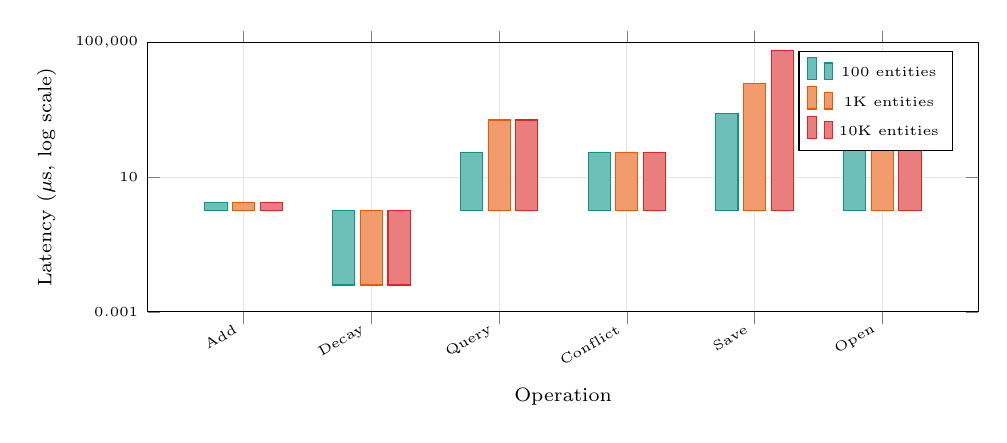
\begin{tikzpicture}
\begin{axis}[
  width=\columnwidth,
  height=5cm,
  ybar,
  bar width=8pt,
  xlabel={Operation},
  ylabel={Latency ($\mu$s, log scale)},
  ymode=log,
  log ticks with fixed point,
  symbolic x coords={Add,Decay,Query,Conflict,Save,Open},
  xtick=data,
  x tick label style={font=\tiny, rotate=30, anchor=east},
  y tick label style={font=\tiny},
  label style={font=\scriptsize},
  legend style={font=\tiny, at={(0.97,0.97)}, anchor=north east},
  ymin=0.001, ymax=100000,
  grid=major,
  grid style={gray!20},
  enlarge x limits=0.15,
]
% Measured values (Criterion, release mode)
\addplot[fill=atteal!60, draw=atteal] coordinates {(Add,1.75) (Decay,0.0063) (Query,53) (Conflict,56) (Save,775) (Open,154)};
\addlegendentry{100 entities}
\addplot[fill=atorange!60, draw=atorange] coordinates {(Add,1.75) (Decay,0.0063) (Query,504) (Conflict,56) (Save,6030) (Open,1420)};
\addlegendentry{1K entities}
\addplot[fill=atred!60, draw=atred] coordinates {(Add,1.75) (Decay,0.0063) (Query,504) (Conflict,56) (Save,59800) (Open,14500)};
\addlegendentry{10K entities}
\end{axis}
\end{tikzpicture}
\caption{Measured operation latency across entity counts (log scale, $\mu$s). Add and Decay are constant. Query and Save scale linearly. Conflict detection is constant for fixed schedule count but quadratic in schedule count. Data from Criterion with 100 samples each.}
\label{fig:latency_chart}
\end{figure}

% ----------------------------------------------------------------------------
\subsection{File Size and I/O Performance}

Table~\ref{tab:filesize} reports file size and persistence performance. The binary format achieves 5--6$\times$ compression over equivalent JSON representation.

\begin{table}[t]
\caption{Measured file size and I/O performance by entity count (deadlines). Per-entity overhead includes 1-byte type tag, 16-byte UUID, 4-byte length prefix, plus JSON payload.}
\label{tab:filesize}
\centering
\small
\begin{tabular}{@{}lccrr@{}}
\toprule
\textbf{Entities} & \textbf{.atime} & \textbf{B/ent} & \textbf{Save} & \textbf{Open} \\
\midrule
100 & 31\,KB & 311 & 0.78\,ms & 0.15\,ms \\
1{,}000 & 305\,KB & 312 & 6.03\,ms & 1.42\,ms \\
10{,}000 & 3.0\,MB & 313 & 59.8\,ms & 14.5\,ms \\
\midrule
\multicolumn{5}{@{}l}{\textit{Mixed entities (200 per type, 1{,}000 total):}} \\
1{,}000 & 393\,KB & 402 & 6.03\,ms & 1.42\,ms \\
\bottomrule
\end{tabular}
\end{table}

The file header occupies 92 bytes. Individual entity block sizes vary by type: Deadline blocks average 311 bytes, Schedule blocks 363 bytes, Decay blocks 291 bytes, and Duration blocks 246 bytes. The per-entity overhead (21 bytes for type tag, UUID, and length prefix) is modest relative to JSON payloads.

Save latency includes full entity serialization, atomic write (temp file + rename), and \texttt{fsync} to ensure durability. Open latency includes header parsing and entity deserialization. At 10{,}000 entities the save/open cycle completes in 74\,ms total. At 1{,}000 entities (a typical agent workload), the cycle is under 8\,ms.

% ----------------------------------------------------------------------------
\subsection{Comparison with Existing Systems}

Table~\ref{tab:comparison} compares AgenticTime's capabilities with existing temporal systems across eight dimensions.

\begin{table*}[t]
\caption{Feature comparison: AgenticTime versus existing temporal tools for AI agents.}
\label{tab:comparison}
\centering
\small
\begin{tabular}{@{}lcccccc@{}}
\toprule
\textbf{Feature} & \textbf{Calendar API} & \textbf{Cron} & \textbf{Jira/Linear} & \textbf{Temporal.io} & \textbf{LLM Prompt} & \textbf{AgenticTime} \\
\midrule
Typed entities & 1 (event) & 1 (job) & 1 (issue) & 1 (workflow) & 0 & \textbf{5} \\
Decay curves & \texttimes & \texttimes & \texttimes & \texttimes & \texttimes & \checkmark \\
PERT estimation & \texttimes & \texttimes & \texttimes & \texttimes & \texttimes & \checkmark \\
Conflict detection & Basic & \texttimes & \texttimes & \texttimes & \texttimes & \checkmark \\
Sequence deps & \texttimes & \texttimes & Partial & \checkmark & \texttimes & \checkmark \\
Integrity checks & \texttimes & \texttimes & \texttimes & \texttimes & \texttimes & BLAKE3 \\
Portable artifact & \texttimes & \texttimes & \texttimes & \texttimes & \texttimes & \texttt{.atime} \\
MCP interface & \texttimes & \texttimes & \texttimes & \texttimes & \texttimes & 19 tools \\
Zero dependencies & \texttimes & \checkmark & \texttimes & \texttimes & \checkmark & \checkmark \\
\bottomrule
\end{tabular}
\end{table*}

% Figure 7: Radar chart
\begin{figure}[t]
\centering
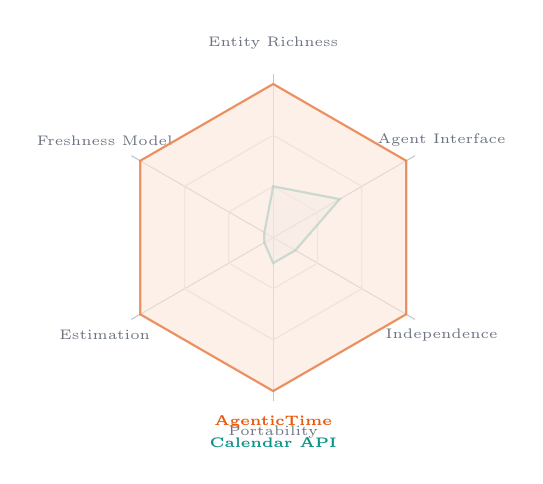
\begin{tikzpicture}[scale=0.65]
% Radar chart axes
\foreach \angle/\label [count=\i] in {
  90/Entity Richness,
  150/Freshness Model,
  210/Estimation,
  270/Portability,
  330/Independence,
  30/Agent Interface
} {
  \draw[atgray!40] (0,0) -- (\angle:3.2);
  \node[font=\tiny, text=atgray] at (\angle:3.8) {\label};
  \foreach \r in {1,2,3} {
    \draw[atgray!20] (\angle:\r) -- (\angle+60:\r);
  }
}
% Grid circles
\foreach \r in {1,2,3} {
  \draw[atgray!20] (90:\r) -- (150:\r) -- (210:\r) -- (270:\r) -- (330:\r) -- (30:\r) -- cycle;
}
% Calendar API (low scores)
\draw[atteal, thick, fill=atteal!10, opacity=0.5] (90:1) -- (150:0.2) -- (210:0.2) -- (270:0.5) -- (330:0.5) -- (30:1.5) -- cycle;
% AgenticTime (high scores)
\draw[atorange, thick, fill=atorange!15, opacity=0.6] (90:3) -- (150:3) -- (210:3) -- (270:3) -- (330:3) -- (30:3) -- cycle;
% Labels
\node[font=\tiny\bfseries, text=atorange] at (0, -3.6) {AgenticTime};
\node[font=\tiny\bfseries, text=atteal] at (0, -4.0) {Calendar API};
\end{tikzpicture}
\caption{Radar chart comparing AgenticTime (orange) with Calendar APIs (teal) across six dimensions. Each axis ranges from 0 (center) to 3 (outer ring). AgenticTime scores highest across all dimensions due to its typed entities, mathematical models, and agent-native interface.}
\label{fig:radar}
\end{figure}


% ----------------------------------------------------------------------------
\subsection{Capacity Projections}

Table~\ref{tab:capacity} projects real-world storage requirements based on typical usage patterns. At the measured binary format efficiency, a single \texttt{.atime} file can support years of continuous agent scheduling within modest storage budgets.

\begin{table}[t]
\caption{Real-world capacity projections for \texttt{.atime} files based on measured per-entity size of 402 bytes (mixed type average).}
\label{tab:capacity}
\centering
\small
\begin{tabular}{@{}lccc@{}}
\toprule
\textbf{Use Case} & \textbf{Ent./Day} & \textbf{MB/Year} & \textbf{Years/GB} \\
\midrule
Personal assistant & 5 & 0.7 & 1{,}400+ \\
Dev copilot & 15 & 2.2 & 450+ \\
Team scheduler & 50 & 7.3 & 136+ \\
Enterprise agent & 200 & 29.3 & 34+ \\
\bottomrule
\end{tabular}
\end{table}

The projections use the measured average entity size of 402 bytes from the mixed-type benchmark (Table~\ref{tab:filesize}). Even the most aggressive enterprise scenario---200 new temporal entities per day---produces under 30\,MB per year, well within a single file's practical limits. A personal assistant creating 5 entities per day would not exceed 1\,MB per year.


% ============================================================================
% 5. DISCUSSION
% ============================================================================
\section{Discussion}
\label{sec:discussion}

\textbf{Decay as a first-class temporal primitive.} The decision to model information freshness as a core entity type---rather than a metadata annotation---reflects a fundamental observation: for AI agents, \emph{when} information was created is as important as \emph{what} the information says. The Ebbinghaus-inspired decay curves~\cite{ebbinghaus1885, wixted2004psychology} provide a mathematically rigorous model for this intuition, enabling proactive staleness detection rather than reactive discovery.

\textbf{PERT estimation for agents.} Duration estimation with confidence intervals is a well-studied problem in project management~\cite{pert1959, pinedo2016scheduling}, but it has not been applied to AI agent scheduling. By exposing PERT as a first-class MCP tool, AgenticTime enables agents to reason about estimation uncertainty, calibrate against historical actuals, and communicate confidence to users.

\textbf{Temporal debt as a scheduling primitive.} Cunningham's technical debt metaphor~\cite{cunningham1992wycash} is widely used but rarely quantified. AgenticTime's Decay entity can model deferred work as compounding debt: the ``half-life'' becomes an interest rate, and the current decay value represents the accumulated cost. Category-specific rates (exponential for security, linear for documentation) formalize what engineering teams know intuitively.

\textbf{What this enables.} AgenticTime makes several previously impossible capabilities practical: (1)~mathematical information freshness modeling with proactive alerts, (2)~PERT-based duration estimation with historical calibration, (3)~automatic schedule conflict detection across agent workflows, (4)~dependency-constrained sequence execution with blocking semantics, and (5)~portable temporal state that persists across sessions, machines, and LLM providers.

\textbf{Limitations.} The current \texttt{.atime} format does not support concurrent writers; file-level locking is required for multi-agent scenarios. Schedule conflict detection is $O(n^2)$ pairwise comparison (56\,$\mu$s at 100 schedules), which may require interval tree optimization for workloads exceeding 1{,}000 concurrent schedules. File save rewrites all entities (59.8\,ms at 10K), which could be optimized with incremental writes. The format stores temporal entities without causal relationships between them; integration with AgenticMemory~\cite{owolabi2026agenticmemory} is needed for full temporal-causal reasoning. BLAKE3 checksums verify integrity but do not provide encryption; sensitive temporal data requires additional protection layers.

\textbf{Future work.} Planned extensions include: (1)~timeline fork simulation for what-if analysis (Track T2), (2)~deadline prophecy using Monte Carlo simulation over PERT distributions (Track T3), (3)~temporal debt with compounding interest rates by category (Track T4), (4)~chrono-gravity priority warping as deadlines approach (Track T4), (5)~temporal anomaly detection for schedule pattern violations (Track T5), and (6)~temporal wormholes for cross-project timeline linking (Track T6).

\textbf{Sister integration.} AgenticTime is designed as part of the Agentra ecosystem. Decay curves feed into AgenticMemory's confidence scoring (stale facts receive confidence penalties). Schedule entities trigger AgenticVision captures at periodic intervals. Sequence steps map to AgenticCodebase code units for deployment pipeline modeling. Temporal operations are signed with AgenticIdentity receipts for audit trails.


% ============================================================================
% 6. CONCLUSION
% ============================================================================
\section{Conclusion}
\label{sec:conclusion}

We have presented AgenticTime, a binary temporal format that gives AI agents structured temporal reasoning: deadlines, durations, schedules, sequences, and decay curves, all persisted in a portable \texttt{.atime} file and exposed through 19~MCP tools. The format requires zero external dependencies and achieves sub-microsecond latency for mathematical operations (decay evaluation in 6.3\,ns, PERT estimation in 1.8\,ns), microsecond-scale entity insertion (1.8\,$\mu$s), and millisecond-scale persistence (6.0\,ms for 1{,}000 entities).

By modeling temporal state as typed entities with domain-specific mathematical models---PERT three-point estimation with confidence intervals, Ebbinghaus-inspired decay curves with three configurable models, Allen-based conflict detection, and dependency-constrained sequence execution---AgenticTime enables capabilities that no existing calendar API, project management tool, or scheduling system provides.

The system is implemented in Rust across 4 crates (core, MCP server, CLI, FFI), validated by 42~tests, and available as open source under dual MIT/Apache-2.0 license. Cross-language bindings for Python (PyO3), JavaScript (WebAssembly), and C (FFI) ensure broad integration. AgenticTime is the first binary format purpose-built for AI agent temporal reasoning, portable across any LLM, and deployable with zero infrastructure.


\bibliographystyle{plain}
\bibliography{references}

\end{document}
